% Options for packages loaded elsewhere
\PassOptionsToPackage{unicode}{hyperref}
\PassOptionsToPackage{hyphens}{url}
%
\documentclass[
]{article}
\usepackage{amsmath,amssymb}
\usepackage{iftex}
\ifPDFTeX
  \usepackage[T1]{fontenc}
  \usepackage[utf8]{inputenc}
  \usepackage{textcomp} % provide euro and other symbols
\else % if luatex or xetex
  \usepackage{unicode-math} % this also loads fontspec
  \defaultfontfeatures{Scale=MatchLowercase}
  \defaultfontfeatures[\rmfamily]{Ligatures=TeX,Scale=1}
\fi
\usepackage{lmodern}
\ifPDFTeX\else
  % xetex/luatex font selection
\fi
% Use upquote if available, for straight quotes in verbatim environments
\IfFileExists{upquote.sty}{\usepackage{upquote}}{}
\IfFileExists{microtype.sty}{% use microtype if available
  \usepackage[]{microtype}
  \UseMicrotypeSet[protrusion]{basicmath} % disable protrusion for tt fonts
}{}
\makeatletter
\@ifundefined{KOMAClassName}{% if non-KOMA class
  \IfFileExists{parskip.sty}{%
    \usepackage{parskip}
  }{% else
    \setlength{\parindent}{0pt}
    \setlength{\parskip}{6pt plus 2pt minus 1pt}}
}{% if KOMA class
  \KOMAoptions{parskip=half}}
\makeatother
\usepackage{xcolor}
\usepackage[margin=1in]{geometry}
\usepackage{graphicx}
\makeatletter
\def\maxwidth{\ifdim\Gin@nat@width>\linewidth\linewidth\else\Gin@nat@width\fi}
\def\maxheight{\ifdim\Gin@nat@height>\textheight\textheight\else\Gin@nat@height\fi}
\makeatother
% Scale images if necessary, so that they will not overflow the page
% margins by default, and it is still possible to overwrite the defaults
% using explicit options in \includegraphics[width, height, ...]{}
\setkeys{Gin}{width=\maxwidth,height=\maxheight,keepaspectratio}
% Set default figure placement to htbp
\makeatletter
\def\fps@figure{htbp}
\makeatother
\setlength{\emergencystretch}{3em} % prevent overfull lines
\providecommand{\tightlist}{%
  \setlength{\itemsep}{0pt}\setlength{\parskip}{0pt}}
\setcounter{secnumdepth}{-\maxdimen} % remove section numbering
\usepackage{fontspec}
\usepackage{xeCJK}
\ifLuaTeX
  \usepackage{selnolig}  % disable illegal ligatures
\fi
\usepackage{bookmark}
\IfFileExists{xurl.sty}{\usepackage{xurl}}{} % add URL line breaks if available
\urlstyle{same}
\hypersetup{
  pdftitle={TSA final project},
  hidelinks,
  pdfcreator={LaTeX via pandoc}}

\title{TSA final project}
\author{}
\date{\vspace{-2.5em}}

\begin{document}
\maketitle

\begin{verbatim}
## 
## Attaching package: 'lubridate'
\end{verbatim}

\begin{verbatim}
## The following objects are masked from 'package:base':
## 
##     date, intersect, setdiff, union
\end{verbatim}

\begin{verbatim}
## Registered S3 method overwritten by 'quantmod':
##   method            from
##   as.zoo.data.frame zoo
\end{verbatim}

\begin{verbatim}
## -- Attaching core tidyverse packages ------------------------ tidyverse 2.0.0 --
## v dplyr   1.1.4     v stringr 1.5.1
## v forcats 1.0.0     v tibble  3.2.1
## v purrr   1.0.2     v tidyr   1.3.1
## v readr   2.1.5     
## -- Conflicts ------------------------------------------ tidyverse_conflicts() --
## x dplyr::filter() masks stats::filter()
## x dplyr::lag()    masks stats::lag()
## i Use the conflicted package (<http://conflicted.r-lib.org/>) to force all conflicts to become errors
## Loading required package: greybox
## 
## Package "greybox", v2.0.8 loaded.
## 
## 
## 
## Attaching package: 'greybox'
## 
## 
## The following object is masked from 'package:tidyr':
## 
##     spread
## 
## 
## The following object is masked from 'package:lubridate':
## 
##     hm
## 
## 
## This is package "smooth", v4.4.0
\end{verbatim}

\section{Introduction, Motivation, Relevance,
Objectives}\label{introduction-motivation-relevance-objectives}

\section{Introduction}\label{introduction}

Electricity demand forecasting is an essential foundation for power grid
operation and planning, especially given the growing frequency of
extreme weather events caused by climate change. The California
Independent System Operator (CAISO), headquartered in Folsom,
California, manages one of the largest electricity markets in the United
States and serves over 32 million users within its regulated area. Each
year, CAISO would deliver more than 260 million megawatt-hours of
electricity (CAISO, n.d.). From 2014 to 2024, the annual peak demand of
CAISO ranges between 43,789 and 51,479 MW (CAISO, 2025), but during the
September 2022 extreme heat wave, it surged to an all-time record of
52,061 MW, releasing an emergency energy alert and affecting over
500,000 customers for potential outage concerns (Kavya Balaraman, 2022).

This record-breaking load not only requires greater precision and
accuracy in real-time grid balancing but also poses significant
challenges for demand forecasting models. Because commonly used linear
models may fail to adequately capture the nonlinear relationship between
temperature and demand, and this underestimation could be expanded
during heat wave periods (Wang et al., 2021). Therefore, motivated by
this concern, our final project analyzes how different time-series
models can forecast electricity demand in CAISO using historical
temperature data from California, especially during heatwave periods.
Specifically, we adopt the SARIMA modeling framework as our baseline and
progressively incorporate temperature and an extreme heat indicator as
exogenous variables. This incremental design helps us to systematically
evaluate how precisely each variable contributes to forecast accuracy.

\section{Motivation}\label{motivation}

Since the 1900s, the average temperature in California has risen by
around 2.5 to 3 degrees, and the frequency of heat waves in the United
States has doubled since the 1980s (Klivans, 2024). At the same time,
compared to the 1960s, in 2024, the average length of the heat wave
seasons has increased by 46 days (Center for Climate And Energy
Solutions, 2025). Therefore, the significantly increasing extreme heat
waves pose a direct threat to the reliability of the power grid.

In recent years, CAISO has been significantly affected by extreme heat,
and among these impacts, three major events illustrate the scale of the
impact.

First, in August 2020, CAISO experienced several rolling blackouts, with
around 492,000 customers losing power for 15 to 150 minutes on August
14, followed by another 321,000 customers losing power for 8 to 90
minutes on August 15 (California ISO, 2020). These rotating outages were
mainly caused by improper planning and preparation, early-evening supply
gaps during solar ramp-down, and CAISO energy trading market issues
related to convergence bidding (California ISO, 2020).

Second, in September 2022, heat waves pushed CAISO peak load to an
all-time record of 52,061 MW (California ISO, 2022), and the demand
across the entire Western Interconnection hit 167,500 MW (California
ISO, 2024). In response, CAISO issued Flex Alerts for 10 consecutive
days and triggered a Stage 3 Energy Emergency Alert to avoid rolling
blackouts (EIA, 2023). According to EIA (2022), natural gas surged to
60\% of the fuel mix, up from around 30\% under normal conditions, to
meet this electricity demand.

Lastly, on July 11, 2024, CAISO demand reached a peak of 43,969 MW, and
the heat wave brought over two weeks of triple-digit temperatures
(100°F+). Because CAISO added 11,000 MW of clean energy resources and
battery storage to the grid, it successfully managed the event without
issuing any Flex Alerts or emergency alerts (Subakti, 2024).

Together, these three events demonstrate the importance of accurate
demand forecasting for supporting resource planning and operational
decisions under extreme heat waves.

\section{Data Set Description}\label{data-set-description}

\begin{verbatim}
##         date daily_avg_load daily_peak_load n_hours tavg_mean tmax_mean
## 1 2021-01-01       21014.04        25383.37      24  41.01342  54.78114
## 2 2021-01-02       21735.53        26164.46      24  42.28283  52.69366
## 3 2021-01-03       21253.75        26062.17      24  43.83502  54.48227
## 4 2021-01-04       23401.97        27650.16      24  43.54882  54.97002
## 5 2021-01-05       23556.94        27810.35      24  42.16779  56.23684
## 6 2021-01-06       24105.09        27934.26      24  43.52189  56.60384
##   tmin_mean tobs_mean n_stations
## 1  33.80783  42.02326       1122
## 2  37.01585  42.92697       1202
## 3  39.38256  44.34302       1184
## 4  37.99295  43.70000       1216
## 5  35.35852  41.37363       1210
## 6  36.36364  41.93617       1125
\end{verbatim}

\section{Methods}\label{methods}

Dataset split: Prior to being utilized for modeling purposes, the data
set was divided into two separate time frames: A training time frame
(2021-2024); and a validation time frame (2025).

Variable Selection: We selected daily peak load as the target variable
because electricity system planning and capacity decisions are driven by
peak demand rather than average demand. This reflects system stress
during high-demand periods, which is more relevant for grid reliability.

Temperature (tmax\_mean) is included as the primary exogenous variable,
as it directly represents peak daily heat exposure and that leads to
high electricity demand for cooling.

To further capture potential nonlinear effects caused by occasional
heatwave events, we constructed a dummy variable as an extreme heat
indicator using the 95th percentile of temperature
(\textasciitilde92°F).

Model 1: SARIMA (Baseline Model) We utilized a SARIMA model as our
baseline model, using only historic electricity demand data to identify
autoregressive structure within the data and weekly seasonality,

Model 2: SARIMAX (with Temperature)

Model 2 includes daily mean maximum temperature as an additional
explanatory variable to the SARIMA model. The inclusion of temperature
as a predictor (xreg) will enable us to model the continuously changing
relationship between temperature and electric energy usage.

Model 3: SARIMAX (with Temperature \& Extreme Heat) Both temperature and
extreme heat indicator were included as predictors in model 3. This
allows us to assess both continuous changes in electric energy
consumption resulting from temperature changes along with possible
discrete increases in electric energy consumption resulting from extreme
heat events.

Model 4: TBATS The SARIMA-based models are limited to capturing a single
seasonal cycle. To address this, we applied TBATS, which is designed to
handle multiple seasonal patterns simultaneously. We specified two
seasonal periods --- weekly (period = 7) and annual (period = 365.25)
--- to reflect both day-of-week variation and summer demand peaks. The
model automatically selects its parameters, including Box-Cox
transformation and ARMA orders, by minimizing AICc. Since TBATS does not
support exogenous regressors, no temperature variable was included.

Model 5: Dynamic Harmonic Regression (DHR) with Temperature Dynamic
Harmonic Regression models seasonality using Fourier terms --- pairs of
sine and cosine waves --- rather than seasonal differencing. This
approach is more flexible and can capture both weekly (period = 7) and
annual (period = 365.25) seasonal patterns simultaneously. The number of
Fourier pairs (K) for each cycle was selected by minimizing AICc,
searching K = 1--3 for the weekly cycle and K = 1--5 for the annual
cycle. Daily mean maximum temperature (tmax\_mean) was also included as
an exogenous regressor, consistent with Models 2 and 3. The underlying
ARIMA order was determined automatically using auto.arima() with
seasonal = FALSE, since the Fourier terms fully handle the seasonal
component.

Model Assessment Each model's prediction accuracy was measured using
RMSE, MAE, and MAPE. The use of these three measurements allowed us to
compare both the absolute performance of each model as well as their
relative performance.

\section{Result}\label{result}

\subsection{Model 1 (Baseline): SARIMA}\label{model-1-baseline-sarima}

\begin{verbatim}
## Series: train_ts 
## ARIMA(2,0,1)(2,0,0)[7] with non-zero mean 
## 
## Coefficients:
##          ar1      ar2     ma1    sar1    sar2        mean
##       0.9828  -0.1664  0.2936  0.2669  0.4093  30042.1503
## s.e.  0.0642   0.0606  0.0636  0.0250  0.0240    761.3743
## 
## sigma^2 = 1863751:  log likelihood = -12620.19
## AIC=25254.38   AICc=25254.45   BIC=25291.38
## 
## Training set error measures:
##                    ME     RMSE      MAE      MPE     MAPE      MASE
## Training set 2.334028 1362.386 973.8017 -0.19916 3.135236 0.4216024
##                       ACF1
## Training set -0.0002581047
\end{verbatim}

\begin{verbatim}
##                       ME     RMSE       MAE       MPE      MAPE     MASE
## Training set    2.334028 1362.386  973.8017 -0.199160  3.135236 0.760041
## Test set     -214.823996 4245.628 3364.6181 -2.643435 11.185134 2.626046
##                       ACF1
## Training set -0.0002581047
## Test set                NA
\end{verbatim}

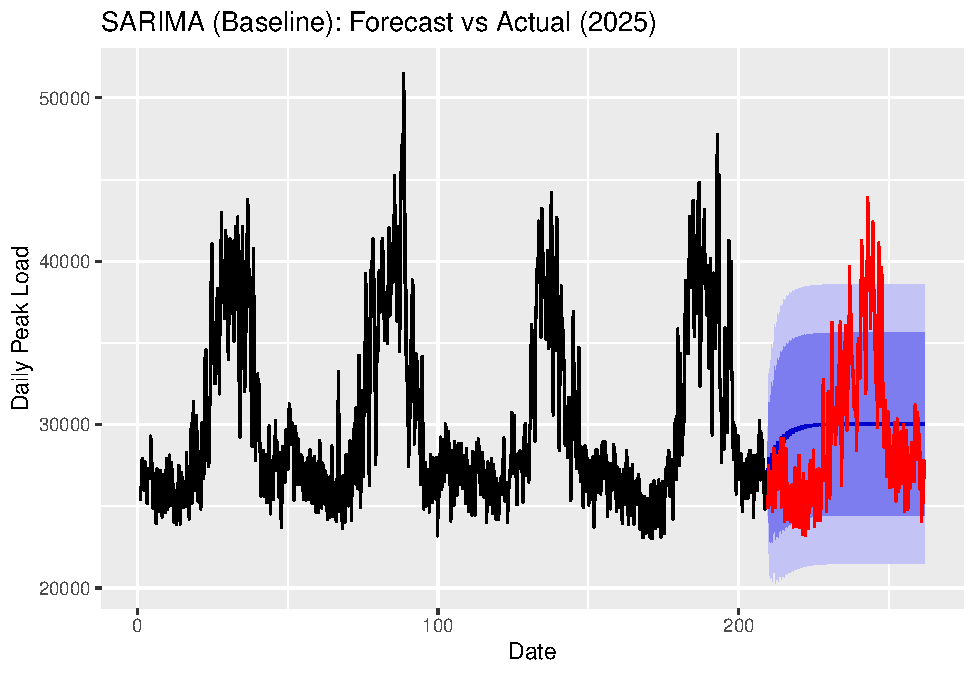
\includegraphics{TSA2026_final-project_files/figure-latex/unnamed-chunk-4-1.pdf}

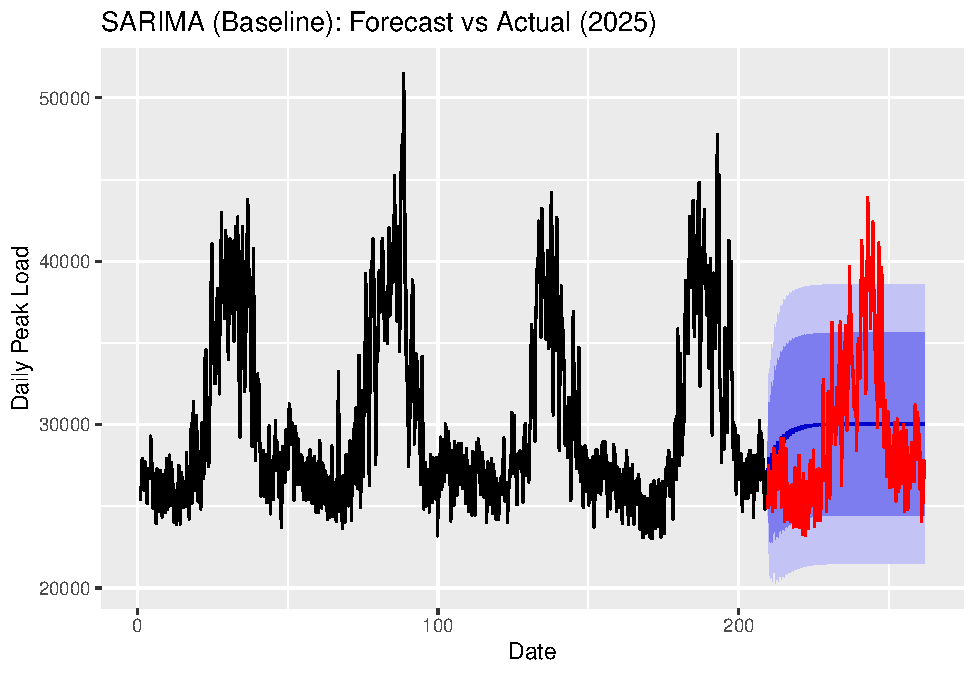
\includegraphics{TSA2026_final-project_files/figure-latex/unnamed-chunk-5-1.pdf}

\subsection{Model 2: SARIMAX}\label{model-2-sarimax}

\begin{verbatim}
## [1] 0
\end{verbatim}

\begin{verbatim}
## [1] 0
\end{verbatim}

\begin{verbatim}
## Series: train_ts 
## Regression with ARIMA(1,0,1)(2,0,0)[7] errors 
## 
## Coefficients:
##          ar1     ma1    sar1    sar2  intercept      xreg
##       0.7650  0.3875  0.2775  0.3891   17929.61  172.5244
## s.e.  0.0193  0.0268  0.0243  0.0243     932.59   10.4954
## 
## sigma^2 = 1588151:  log likelihood = -12502.99
## AIC=25019.99   AICc=25020.06   BIC=25057
## 
## Training set error measures:
##                     ME     RMSE      MAE        MPE     MAPE      MASE
## Training set 0.1371501 1257.628 936.7978 -0.1841657 3.073758 0.4055818
##                     ACF1
## Training set 0.006579419
\end{verbatim}

\begin{verbatim}
##                        ME     RMSE       MAE        MPE     MAPE      MASE
## Training set    0.1371501 1257.628  936.7978 -0.1841657 3.073758 0.7311599
## Test set     -534.4727405 3014.653 2378.6382 -3.0226593 8.068820 1.8564998
##                     ACF1
## Training set 0.006579419
## Test set              NA
\end{verbatim}

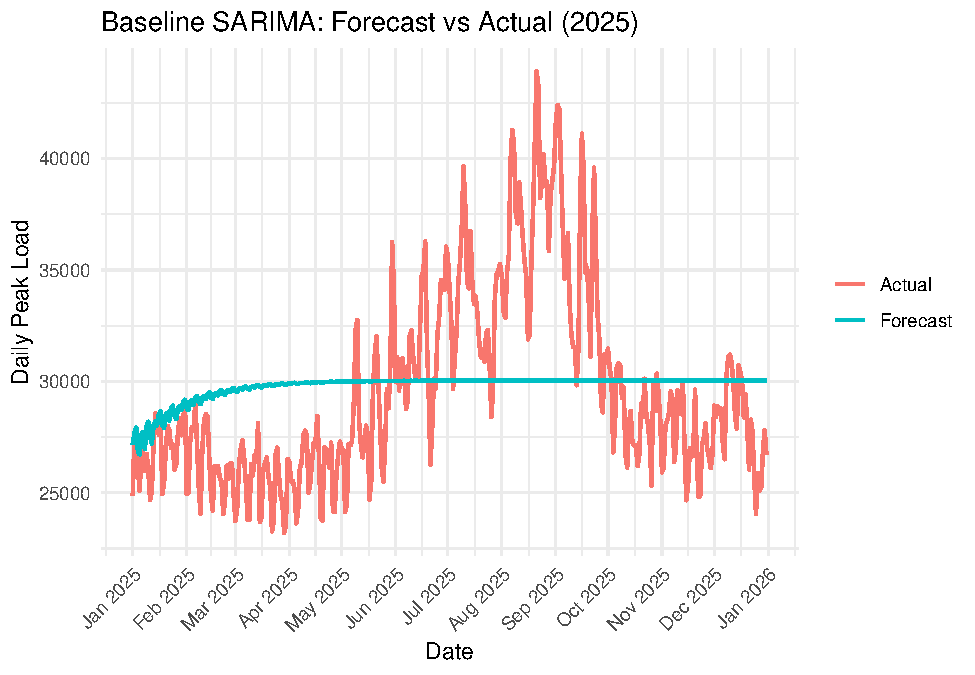
\includegraphics{TSA2026_final-project_files/figure-latex/unnamed-chunk-6-1.pdf}

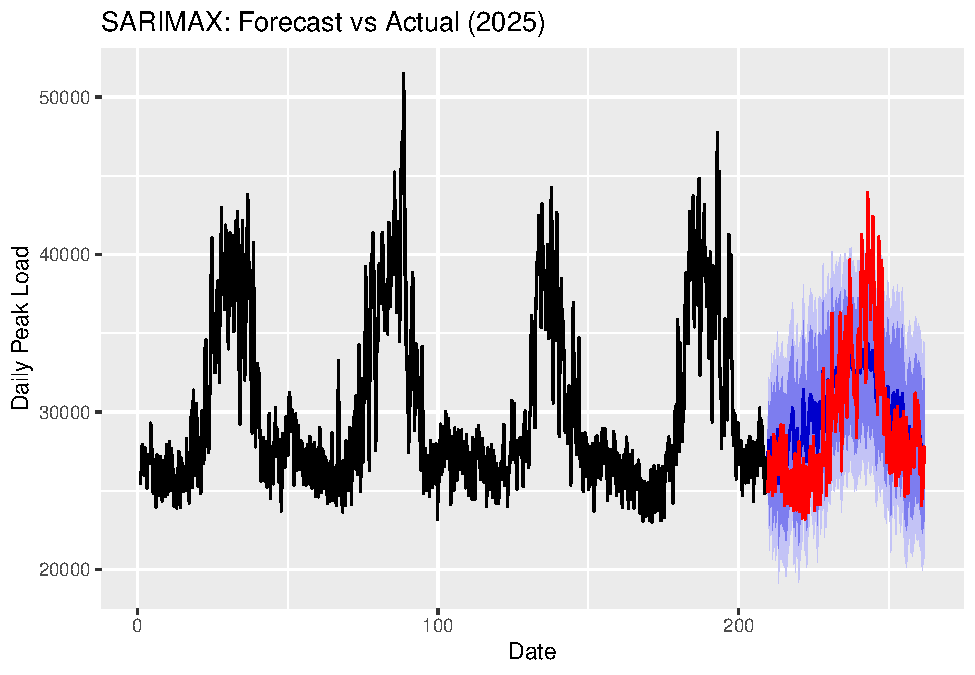
\includegraphics{TSA2026_final-project_files/figure-latex/unnamed-chunk-7-1.pdf}

\subsection{Model 3: Sarimax + Extreme heat
dummy}\label{model-3-sarimax-extreme-heat-dummy}

\begin{verbatim}
## 
##    0    1 
## 1764   93
\end{verbatim}

\begin{verbatim}
##      95% 
## 91.95149
\end{verbatim}

\begin{verbatim}
## Series: train_ts 
## Regression with ARIMA(1,0,1)(2,0,0)[7] errors 
## 
## Coefficients:
##          ar1     ma1    sar1    sar2   intercept      tmax   extreme
##       0.7589  0.3686  0.2853  0.3917  18261.1733  167.1146  849.3532
## s.e.  0.0198  0.0280  0.0243  0.0242    919.0036   10.3632  177.2899
## 
## sigma^2 = 1564226:  log likelihood = -12491.45
## AIC=24998.89   AICc=24998.99   BIC=25041.19
## 
## Training set error measures:
##                     ME    RMSE      MAE        MPE    MAPE      MASE
## Training set 0.1421097 1247.69 926.5318 -0.1851644 3.04019 0.4011372
##                     ACF1
## Training set 0.003576836
\end{verbatim}

\begin{verbatim}
##                        ME    RMSE       MAE        MPE     MAPE      MASE
## Training set    0.1421097 1247.69  926.5318 -0.1851644 3.040190 0.7231474
## Test set     -495.5923634 2996.04 2365.5567 -2.8936806 8.017726 1.8462898
##                     ACF1
## Training set 0.003576836
## Test set              NA
\end{verbatim}

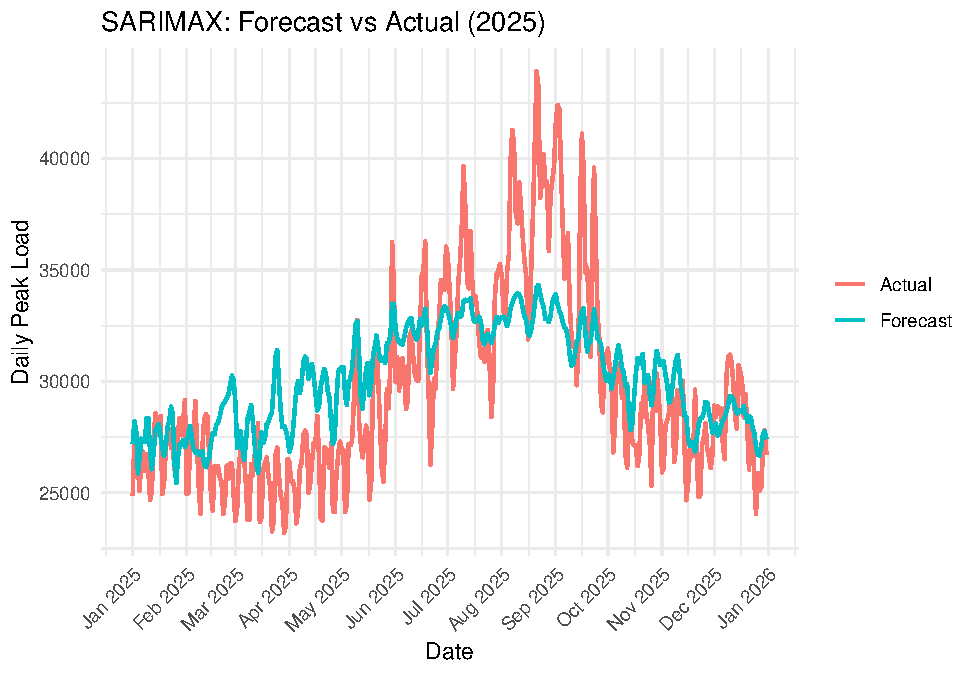
\includegraphics{TSA2026_final-project_files/figure-latex/unnamed-chunk-8-1.pdf}

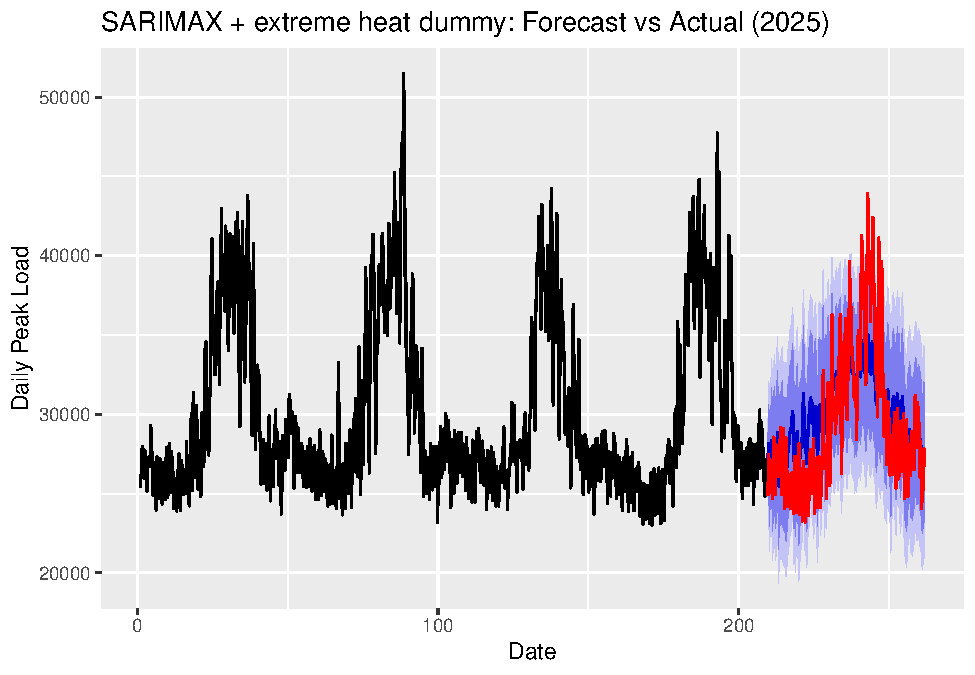
\includegraphics{TSA2026_final-project_files/figure-latex/unnamed-chunk-9-1.pdf}

\subsection{Model 4: TBATS}\label{model-4-tbats}

\begin{verbatim}
##                   Length Class  Mode     
## lambda                1  -none- numeric  
## alpha                 1  -none- numeric  
## beta                  1  -none- numeric  
## damping.parameter     1  -none- numeric  
## gamma.one.values      2  -none- numeric  
## gamma.two.values      2  -none- numeric  
## ar.coefficients       4  -none- numeric  
## ma.coefficients       2  -none- numeric  
## likelihood            1  -none- numeric  
## optim.return.code     1  -none- numeric  
## variance              1  -none- numeric  
## AIC                   1  -none- numeric  
## parameters            2  -none- list     
## seed.states          28  -none- numeric  
## fitted.values      1461  msts   numeric  
## errors             1461  msts   numeric  
## x                 40908  -none- numeric  
## seasonal.periods      2  -none- numeric  
## k.vector              2  -none- numeric  
## y                  1461  msts   numeric  
## p                     1  -none- numeric  
## q                     1  -none- numeric  
## call                  2  -none- call     
## series                1  -none- character
## method                1  -none- character
\end{verbatim}

\begin{verbatim}
##                      ME     RMSE       MAE         MPE     MAPE      MASE
## Training set   11.41163 1174.472  801.5045 -0.07250059 2.565443 0.6255651
## Test set     1633.35565 2792.698 2157.1653  5.22164394 6.983400 1.6836428
##                    ACF1
## Training set 0.05395752
## Test set             NA
\end{verbatim}

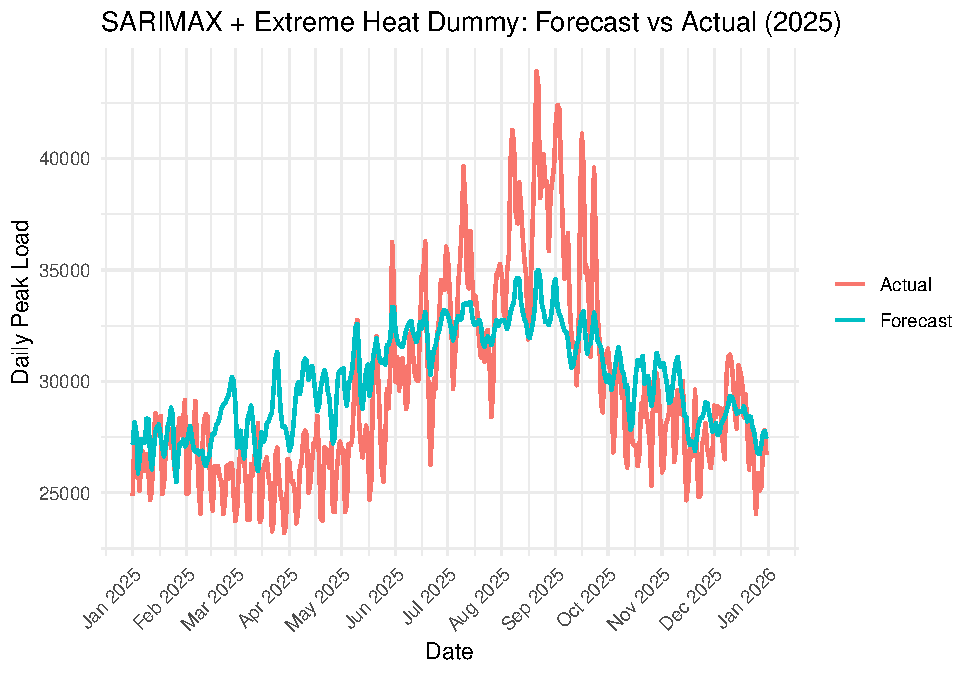
\includegraphics{TSA2026_final-project_files/figure-latex/unnamed-chunk-10-1.pdf}
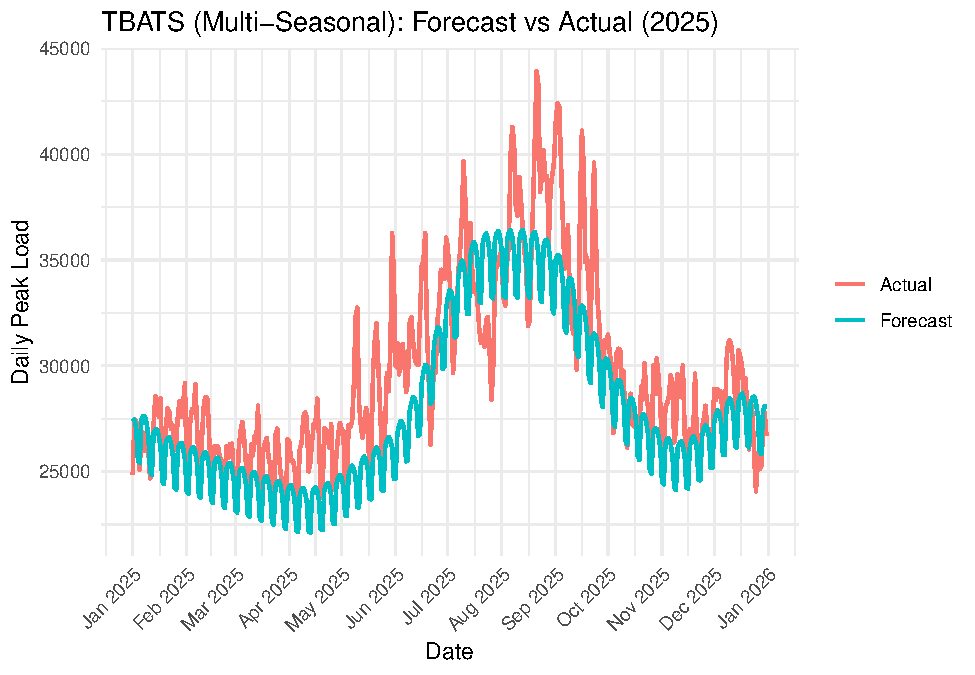
\includegraphics{TSA2026_final-project_files/figure-latex/unnamed-chunk-10-2.pdf}

\subsection{Model 5: Dynamic Harmonic Regression (ARIMA + Fourier
Terms)}\label{model-5-dynamic-harmonic-regression-arima-fourier-terms}

\begin{verbatim}
## K = 1 1 | AICc = 25174.67 
## K = 1 2 | AICc = 25069.24 
## K = 1 3 | AICc = 25071.32 
## K = 1 4 | AICc = 25072.95 
## K = 1 5 | AICc = 25075.24 
## K = 2 1 | AICc = 24868.6 
## K = 2 2 | AICc = 24808.58 
## K = 2 3 | AICc = 24788.16 
## K = 2 4 | AICc = 24790.4 
## K = 2 5 | AICc = 24792.96 
## K = 3 1 | AICc = 24702.24 
## K = 3 2 | AICc = 24648.22 
## K = 3 3 | AICc = 24632.95 
## K = 3 4 | AICc = 24635.27 
## K = 3 5 | AICc = 24637.86
\end{verbatim}

\begin{verbatim}
## 
## Best K: 3 3
\end{verbatim}

\begin{verbatim}
## Series: train_msts 
## Regression with ARIMA(1,0,1) errors 
## 
## Coefficients:
##          ar1     ma1   intercept       S1-7      C1-7      S2-7      C2-7
##       0.7273  0.3915  18339.7572  -1215.936  709.0534  600.3234  115.2949
## s.e.  0.0206  0.0274    726.2614     65.855   65.8523   29.4622   29.4576
##            S3-7       C3-7      S1-365      C1-365     S2-365     C2-365
##       -197.4392  -129.4222  -2329.3427  -1622.2355  2336.4499  1323.8959
## s.e.    16.0972    16.1284    220.3231    262.2166   207.0332   204.7627
##          S3-365    C3-365      tmax
##       -850.7799  359.5537  166.5803
## s.e.   204.1449  203.2951   10.0839
## 
## sigma^2 = 1212512:  log likelihood = -12298.73
## AIC=24631.46   AICc=24631.88   BIC=24721.33
## 
## Training set error measures:
##                    ME     RMSE      MAE        MPE     MAPE      MASE
## Training set 1.671478 1095.095 791.6652 -0.1027929 2.592962 0.3196913
##                     ACF1
## Training set 0.004859625
\end{verbatim}

\begin{verbatim}
##                       ME     RMSE       MAE        MPE     MAPE      MASE
## Training set    1.671478 1095.095  791.6652 -0.1027929 2.592962 0.6178856
## Test set     -584.266991 2100.466 1554.7297 -2.1150226 5.145530 1.2134487
##                     ACF1
## Training set 0.004859625
## Test set              NA
\end{verbatim}

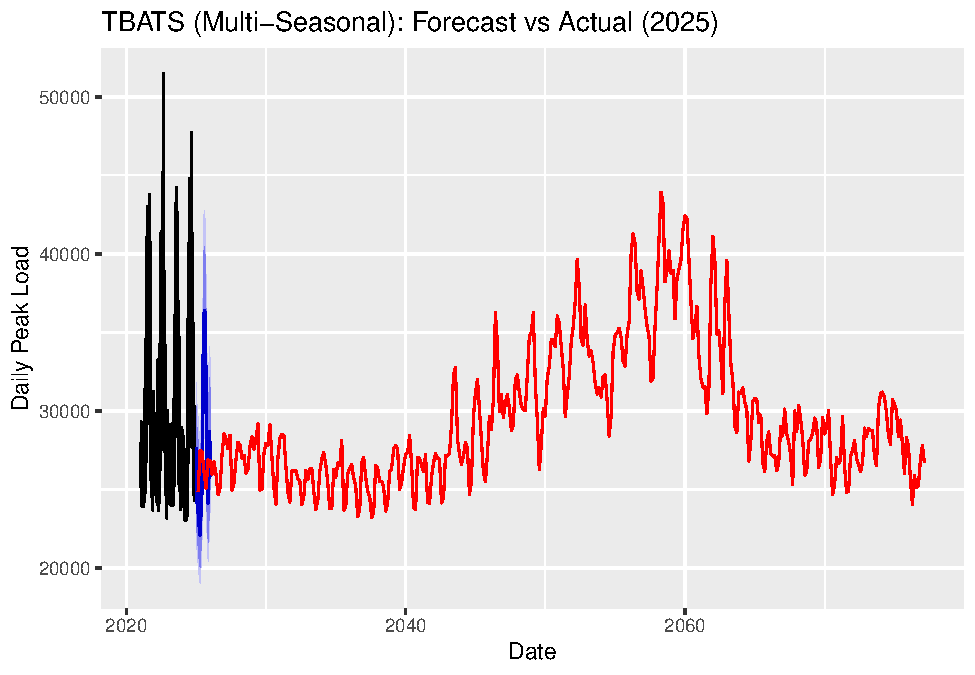
\includegraphics{TSA2026_final-project_files/figure-latex/unnamed-chunk-11-1.pdf}

\subsection{Model comparison}\label{model-comparison}

\begin{verbatim}
##                  Model    RMSE Rank
## 1           DHR + tmax 2100.47    1
## 2                TBATS 2792.70    2
## 3 SARIMAX + Heat Dummy 2996.04    3
## 4              SARIMAX 3014.65    4
## 5    SARIMA (Baseline) 4245.63    5
\end{verbatim}

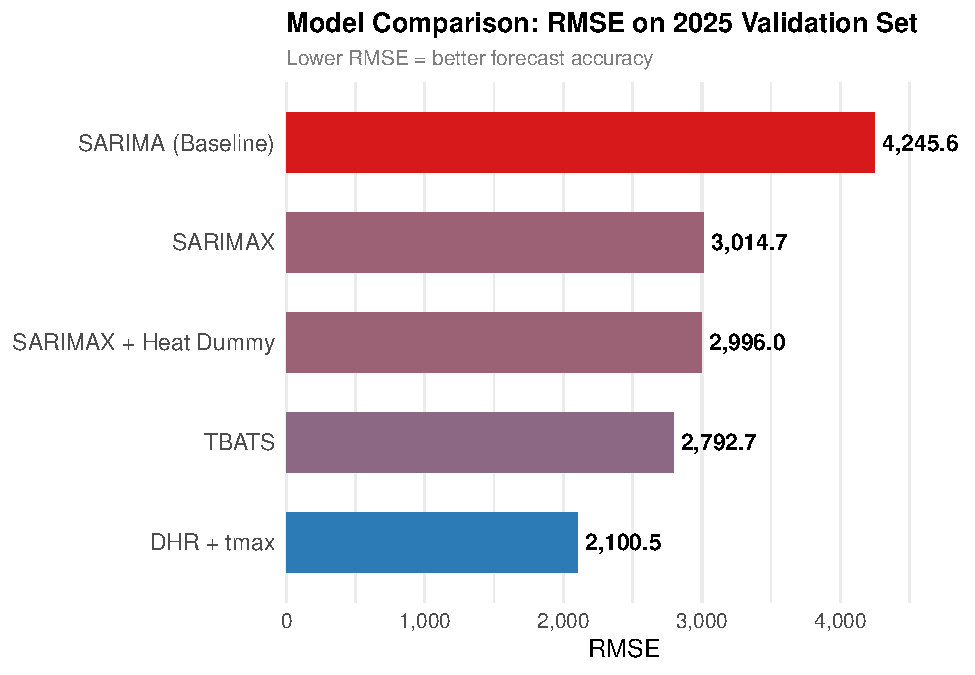
\includegraphics{TSA2026_final-project_files/figure-latex/unnamed-chunk-12-1.pdf}
\# Results The results for 2025 show that incorporating temperature
significantly improves forecasting accuracy. The SARIMAX model reduces
RMSE from 4245.6 to 3014.7 (approximately 29\% improvement), with
similar improvements in MAE and MAPE. This confirms that electricity
demand in CAISO is strongly driven by temperature, as higher
temperatures increase cooling demand and lead to higher electricity
load.

However, adding the extreme heat dummy provides only marginal additional
improvement (RMSE: 3014.7 → 2996.0). This suggests that the continuous
temperature variable already captures most of the variation in demand,
including during heatwave periods. Overall, the results indicate that
electricity demand responds smoothly to temperature changes rather than
rare extreme heatwave events.

When comparing all models, those that incorporate more flexible seasonal
structures perform substantially better. The TBATS model, which captures
both weekly and annual seasonality, further reduces the RMSE to 2792.7,
outperforming all SARIMA-based models. This highlights the importance of
modeling multiple seasonal patterns in electricity demand data, which
cannot be fully captured by standard seasonal differencing alone.

The best-performing model is the Dynamic Harmonic Regression (DHR) with
temperature, achieving the lowest RMSE of 2100.5. This represents a
significant improvement over all other models, including TBATS. The
superior performance of the DHR model suggests that combining Fourier
terms to model complex seasonal patterns with temperature as an
exogenous variable provides the most accurate forecasts. In particular,
the DHR model is able to flexibly capture both short-term (weekly) and
long-term (annual) seasonality while also accounting for
temperature-driven demand fluctuations.

Overall, the results demonstrate a clear ranking of model performance,
with DHR + temperature performing best, followed by TBATS, SARIMAX-based
models, and finally the baseline SARIMA model. These findings emphasize
that both exogenous variables (such as temperature) and advanced
seasonal modeling techniques are essential for improving electricity
demand forecasts.

\section{Discussion}\label{discussion}

The results of this study provide strong evidence that incorporating
temperature as an exogenous variable significantly improves the accuracy
of electricity demand forecasting models. Comparing the baseline SARIMA
model with the SARIMAX variants clearly shows that models relying solely
on historical load data fail to capture key external drivers,
particularly weather conditions. The large reduction in RMSE from
4245.63 (SARIMA) to approximately 3014 (SARIMAX) highlights the
importance of temperature as a primary determinant of electricity demand
in California. The addition of the extreme heat dummy variable resulted
in only a marginal improvement in forecasting performance, suggesting
that the relationship between temperature and electricity demand is
largely continuous rather than driven by discrete threshold effects. In
other words, demand appears to increase progressively with temperature
rather than spiking only during extreme heat events. This finding aligns
with the idea that cooling demand ramps up steadily as temperatures
rise, rather than changing abruptly at a specific cutoff point.

Among all models tested, the Dynamic Harmonic Regression (DHR) model
with temperature achieved the best performance, with the lowest RMSE of
2100.47. This indicates that capturing complex seasonal patterns---both
weekly and annual---through Fourier terms provides a substantial
advantage over traditional seasonal models like SARIMA and even TBATS.
The DHR model's flexibility allows it to better represent multiple
seasonal cycles and their interaction with temperature, which is
particularly important in electricity demand data characterized by
strong periodic behavior.

The TBATS model also performed relatively well, ranking second, which
further supports the importance of modeling multiple seasonalities.
However, its performance was still notably weaker than DHR, suggesting
that explicitly incorporating temperature alongside flexible seasonality
modeling yields the best results.

In summary, these findings emphasize that accurate electricity demand
forecasting requires both strong representation of seasonal patterns and
inclusion of relevant external variables such as temperature.

\section{Summary and Conclusions}\label{summary-and-conclusions}

This project examined the effectiveness of different time series models
in forecasting electricity demand in California, with a particular focus
on the role of temperature and extreme heat events. Using data from
2021--2024 for training and 2025 for validation, we compared five
models: SARIMA, SARIMAX, SARIMAX with an extreme heat dummy, TBATS, and
Dynamic Harmonic Regression (DHR) with temperature.

The results show a clear ranking of model performance: DHR + temperature
(best performance) TBATS SARIMAX + heat dummy SARIMAX SARIMA (baseline)

Including temperature consistently improved model accuracy, while the
extreme heat indicator provided only limited additional benefit. Models
that accounted for multiple seasonal patterns, especially DHR,
outperformed traditional approaches.

In conclusion, this study demonstrates that temperature is a critical
factor in forecasting electricity demand, and its inclusion
significantly enhances model performance. While extreme heat events are
important from a policy and operational perspective, they do not appear
to add substantial predictive power beyond what is already captured by
continuous temperature variables.

The superior performance of the DHR model suggests that combining
flexible seasonal modeling with exogenous variables is the most
effective approach for electricity demand forecasting. This has
important implications for grid operators like CAISO, as more accurate
forecasts can improve resource planning, reduce the risk of outages, and
enhance system reliability during periods of high demand.

Future research could extend this work by incorporating additional
variables such as humidity, electricity prices, or renewable energy
generation, as well as exploring machine learning approaches to capture
nonlinear relationships more effectively. \# Reference

CAISO. (n.d.). How electricity flows \textbar{} California ISO.
Caiso.com. Retrieved April 24, 2026, from
\url{https://www.caiso.com/about/our-business/how-electricity-flows}

CAISO. (2025). 2025 Summer Loads and Resources Assessment. Caiso.com.
\url{https://www.caiso.com/content/summer-loads-resources-assessment/2025/index.html}

California ISO. (2020). This page intentionally left blank.
\url{https://www.caiso.com/documents/preliminary-root-cause-analysis-rotating-outages-august-2020.pdf}

California ISO. (2022). NEWS RELEASE California ISO posts analysis of
September heat wave.
\url{https://www.caiso.com/Documents/california-iso-posts-analysis-of-september-heat-wave.pdf}

California ISO. (2024). Summer Market Performance Report.
\url{https://www.caiso.com/documents/summer-market-performance-report-july-2024.pdf}

Center for Climate And Energy Solutions. (2025). Heat Waves and Climate
Change. Center for Climate and Energy Solutions; C2ES.
\url{https://www.c2es.org/content/heat-waves-and-climate-change/}

EIA. (2022). California fuel mix changes in response to September heat
wave. Www.eia.gov.
\url{https://www.eia.gov/todayinenergy/detail.php?id=53939}

EIA. (2023). California consumers respond to appeals for electricity
conservation during heat wave - U.S. Energy Information Administration
(EIA). Eia.gov.
\url{https://www.eia.gov/todayinenergy/detail.php?id=54039}

Kavya Balaraman. (2022, September 7). California ISO narrowly avoids
rolling outages as peak demand hits record 52 GW. Utility Dive.
\url{https://www.utilitydive.com/news/california-iso-narrowly-avoids-outages-but-warns-as-peak-demand-hits-record/631280/}

Klivans, L. (2024, October 4). Yes, These California Heat Waves Are
Connected to Climate Change. Here's How. Kqed.org.
\url{https://www.kqed.org/science/1994643/yes-these-california-heat-waves-are-connected-to-climate-change-heres-how}

Subakti, D. (2024, July 15). Managing the July 2024 heat wave with our
partners in California and the West \textbar{} California ISO.
Caiso.com.
\url{https://www.caiso.com/about/news/energy-matters-blog/managing-the-july-2024-heat-wave-with-our-partners-in-california-and-the-west}

Wang, Z., Hong, T., Li, H., \& Ann Piette, M. (2021). Predicting
city-scale daily electricity consumption using data-driven models.
Advances in Applied Energy, 2, 100025.
\url{https://doi.org/10.1016/j.adapen.2021.100025}

\end{document}
